\documentclass{article}
\usepackage{graphicx}
\usepackage{amsmath}
\usepackage{amssymb}
\usepackage{listings}
\usepackage[margin=1in]{geometry}
\usepackage{xcolor}
\usepackage{tikz}
\usetikzlibrary{shapes, arrows, positioning, calc}
\usepackage{tcolorbox}

% Define colors for syntax highlighting
\definecolor{codegreen}{rgb}{0,0.6,0}
\definecolor{codegray}{rgb}{0.5,0.5,0.5}
\definecolor{codepurple}{rgb}{0.58,0,0.82}
\definecolor{backcolour}{rgb}{0.95,0.95,0.92}

% Python style for highlighting
\lstdefinestyle{pythonstyle}{
    backgroundcolor=\color{backcolour},
    commentstyle=\color{codegreen},
    keywordstyle=\color{magenta},
    numberstyle=\tiny\color{codegray},
    stringstyle=\color{codepurple},
    basicstyle=\ttfamily\footnotesize,
    breakatwhitespace=false,
    breaklines=true,
    captionpos=b,
    keepspaces=true,
    numbers=left,
    numbersep=5pt,
    showspaces=false,
    showstringspaces=false,
    showtabs=false,
    tabsize=2
}
\lstset{style=pythonstyle}

\title{Lecture 10: Positional Encoding in Transformers}
\author{Deep Learning Class}
\date{\today}

\begin{document}
    \section{The Positional Encoding Problem: A Geometric Perspective}

We have established that self-attention treats the input as an unordered set. To inject positional information, we need to add a position-dependent signal to each token embedding. But how should we design this signal?

\subsection{The Geometric Constraints from Dot-Product Attention}

Before attempting any solution, we must understand the fundamental constraints imposed by how attention \textit{uses} positional information.

\textbf{The attention mechanism computes dot products:}
\[
\text{score}(q, k) = q^T k = \|q\| \|k\| \cos(\theta)
\]

The dot product has two components:
\begin{itemize}
\item \textbf{Magnitude:} $\|q\| \|k\|$ (the lengths of the vectors)
\item \textbf{Angle:} $\cos(\theta)$ (the cosine of the angle between them)
\end{itemize}

Both components affect the attention score. This imposes critical constraints on how we add positional information.

\begin{tcolorbox}[colback=yellow!5!white, colframe=orange!50!black, title=The Core Design Constraints]
An ideal positional encoding must satisfy:

\textbf{1. Constructive Interaction with Semantics:} Positional information should combine with semantic information without destroying the learned relationships between token embeddings.

\textbf{2. Norm Preservation:} Adding positional encoding should not arbitrarily inflate or deflate the magnitudes of embeddings. If position doubles the norm of some embeddings but not others, position will dominate attention scores unpredictably.

\textbf{3. Linear Transformability:} For the model to easily learn patterns like ``attend to the previous word,'' a shift in position (e.g., from position $i$ to $i+\delta$) should correspond to a \textbf{linear transformation} that is \textbf{independent of the absolute position $i$}.

\textbf{4. Geometric Interpretation:} Relative position relationships should have simple geometric structure that attention can exploit through dot products.
\end{tcolorbox}

\textbf{Why rotations emerge naturally:} Rotations are linear transformations that preserve vector norms. If we design positional encoding such that ``moving forward by $\delta$ positions'' corresponds to a rotation by angle $\delta \omega$, then:
\begin{itemize}
\item The norm is preserved: $\|\mathbf{p}_i\| = \|\mathbf{p}_{i+\delta}\|$
\item The transformation is linear and position-independent
\item The angle change encodes relative position in a way that dot products can measure
\end{itemize}

These constraints will guide our design and ultimately lead us to sinusoidal functions.

\subsection{Design Goals}

An ideal positional encoding scheme should satisfy:

\begin{enumerate}
\item \textbf{Uniqueness:} Each position must have a distinct representation
\item \textbf{Determinism:} The encoding should be reproducible and not random
\item \textbf{Bounded Range:} Values should remain within a reasonable range for numerical stability and to avoid dominating semantic information
\item \textbf{Generalization:} Should work for sequences longer than those seen during training
\item \textbf{Distance Awareness:} The model should distinguish both near and far positions at multiple scales
\item \textbf{Smooth Transitions:} Nearby positions should have similar encodings (continuity for gradient descent)
\item \textbf{Linear Transformability:} Shifting position by $\delta$ (e.g., $i \rightarrow i+\delta$) should correspond to a simple linear transformation that is independent of the starting position $i$. This enables the model to learn position-invariant patterns like ``attend to the previous word.''
\item \textbf{Norm Preservation:} Adding positional encoding should not arbitrarily inflate or deflate embedding magnitudes
\end{enumerate}

Let us now build up a solution that satisfies these requirements.

\section{Attempt 1: Normalized Linear Weights}

\subsection{The Idea}

The simplest approach: assign each position a normalized scalar value between 0 and 1:
\[
p_i = \frac{i}{n-1}
\]
where $i$ is the position index and $n$ is the sequence length.

For a sequence of length 10:
\begin{center}
\begin{tabular}{c|cccccccccc}
Position & 0 & 1 & 2 & 3 & 4 & 5 & 6 & 7 & 8 & 9 \\
\hline
Encoding & 0.00 & 0.11 & 0.22 & 0.33 & 0.44 & 0.56 & 0.67 & 0.78 & 0.89 & 1.00 \\
\end{tabular}
\end{center}

We broadcast this scalar to a $d$-dimensional vector by adding it to all dimensions:
\[
\mathbf{x}_{\text{input}}^{(i)} = \mathbf{e}_i + p_i \cdot \mathbf{1}
\]
where $\mathbf{1} = [1, 1, 1, \ldots, 1]^T \in \mathbb{R}^d$ is the all-ones vector.

\subsection{What Fails: The Geometric Disaster}

\begin{tcolorbox}[colback=red!5!white, colframe=red!75!black, title=Critical Problem: All Positions Point in the Same Direction!]
The fundamental geometric flaw: \textbf{all positional encodings are parallel vectors}.

\textbf{Every position's encoding is a scalar multiple of the same vector $\mathbf{1}$:}
\begin{align}
\text{Position 0:} \quad &p_0 \cdot \mathbf{1} = 0.00 \cdot [1, 1, \ldots, 1]^T \\
\text{Position 5:} \quad &p_5 \cdot \mathbf{1} = 0.56 \cdot [1, 1, \ldots, 1]^T \\
\text{Position 9:} \quad &p_9 \cdot \mathbf{1} = 1.00 \cdot [1, 1, \ldots, 1]^T
\end{align}

These vectors all point in the \emph{same direction} (the diagonal direction where all coordinates are equal). They differ only in magnitude!
\end{tcolorbox}

\subsection{Why This is Catastrophic for Attention}

Recall that attention computes dot products between queries and keys:
\[
\text{score}(i, j) = (\mathbf{e}_i + p_i \mathbf{1})^T (\mathbf{e}_j + p_j \mathbf{1})
\]

Expanding this:
\begin{align}
\text{score}(i, j) &= \mathbf{e}_i^T \mathbf{e}_j + p_i \mathbf{1}^T \mathbf{e}_j + p_j \mathbf{1}^T \mathbf{e}_i + p_i p_j \|\mathbf{1}\|^2 \\
&= \mathbf{e}_i^T \mathbf{e}_j + p_i \sum_{k=1}^d e_{j,k} + p_j \sum_{k=1}^d e_{i,k} + p_i p_j \cdot d
\end{align}

\textbf{The problem:} The positional component is just adding the same global bias to everything:
\begin{itemize}
\item The term $p_i \sum_{k} e_{j,k}$ depends on the sum of ${\mathbf{e}_j}$'s coordinates (a single number per token)
\item The term $p_i p_j \cdot d$ is symmetric and provides minimal distinguishing information
\item There's no rich interaction between position and semantic content
\end{itemize}

\subsection{Geometric Visualization}

\begin{center}
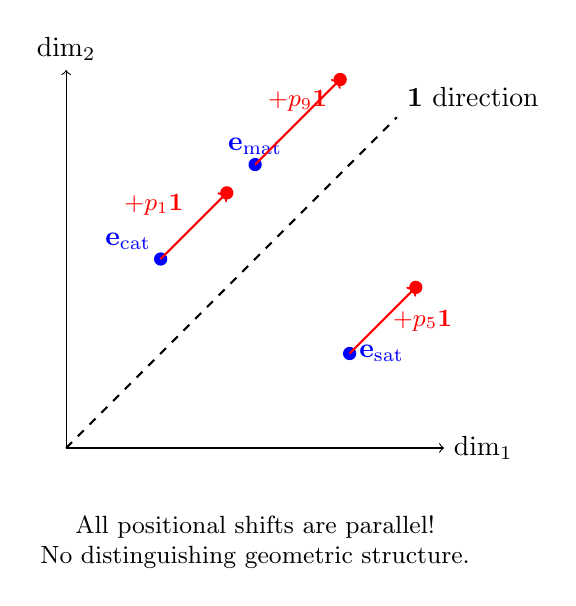
\begin{tikzpicture}[scale=1.2]
% 2D projection for visualization
\draw[->] (0,0) -- (4,0) node[right] {$\dim_1$};
\draw[->] (0,0) -- (0,4) node[above] {$\dim_2$};

% All positional encodings lie on the diagonal (same direction)
\draw[thick, dashed] (0,0) -- (3.5,3.5) node[above right] {$\mathbf{1}$ direction};

% Token embeddings (scattered in space)
\fill[blue] (1,2) circle (2pt) node[above left] {$\mathbf{e}_{\text{cat}}$};
\fill[blue] (3,1) circle (2pt) node[right] {$\mathbf{e}_{\text{sat}}$};
\fill[blue] (2,3) circle (2pt) node[above] {$\mathbf{e}_{\text{mat}}$};

% Adding positional encoding just shifts along diagonal
\draw[->, thick, red] (1,2) -- (1.7,2.7) node[midway, above left, font=\small] {$+p_1 \mathbf{1}$};
\draw[->, thick, red] (3,1) -- (3.7,1.7) node[midway, right, font=\small] {$+p_5 \mathbf{1}$};
\draw[->, thick, red] (2,3) -- (2.9,3.9) node[midway, above, font=\small] {$+p_9 \mathbf{1}$};

\fill[red] (1.7,2.7) circle (2pt);
\fill[red] (3.7,1.7) circle (2pt);
\fill[red] (2.9,3.9) circle (2pt);

\node[align=center, font=\small] at (2, -1) {All positional shifts are parallel!\\No distinguishing geometric structure.};
\end{tikzpicture}
\end{center}

All we're doing is shifting each embedding along the same diagonal direction by different amounts. The \textbf{angles between vectors} (which attention cares about) barely change!

\subsection{Additional Fatal Flaws}

\begin{enumerate}
\item \textbf{Violates norm preservation constraint:} Adding $p_i \mathbf{1}$ drastically alters the norm of each embedding vector:
\[
\|\mathbf{e}_i + p_i \mathbf{1}\|^2 = \|\mathbf{e}_i\|^2 + 2p_i \mathbf{1}^T \mathbf{e}_i + p_i^2 d
\]
The final term grows as $p_i^2 d$. For large $p_i$ (late positions), this can double or triple the embedding norm! Since attention scores depend on both angle \textit{and} magnitude, this unpredictably distorts the learned semantic similarities.

\item \textbf{Violates position-independence constraint:} The encoding depends on sequence length $n$. Position 5 in a 10-token sequence gets $p_5 = 0.56$, but position 5 in a 100-token sequence gets $p_5 = 0.05$. There is no consistent linear transformation representing ``shift by $k$ positions.''

\item \textbf{No directional diversity:} In a $d$-dimensional space, we have $d$ degrees of freedom, but we're only using \emph{one direction} (the $\mathbf{1}$ vector). This is incredibly wasteful of our representational capacity.
\end{enumerate}

\subsection{The Core Lessons}

\begin{tcolorbox}[colback=yellow!5!white, colframe=orange!50!black, title=What We Learned]
To encode position effectively, we need:
\begin{enumerate}
\item \textbf{Directional diversity:} Different positions should point in different directions in the embedding space, not just differ in magnitude along one axis.

\item \textbf{Multi-dimensional structure:} Use the full $d$-dimensional space to encode positional information at multiple scales.

\item \textbf{Rich geometric interactions:} Positional encoding should create meaningful geometric relationships that attention can exploit.
\end{enumerate}

\textbf{The fix:} Instead of one scalar that gets broadcasted, we need a $d$-dimensional vector where each dimension encodes position differently. This leads us to multi-scale representations.
\end{tcolorbox}

\section{Attempt 2: Multi-Scale Binary Encoding}

\subsection{The Inspiration: Binary Numbers}

How do we represent numbers efficiently with multiple granularities? \textbf{Binary representation!}

Consider positions 0 through 7 in 3-bit binary:

\begin{center}
\begin{tabular}{c|ccc|l}
Position & Bit 2 & Bit 1 & Bit 0 & Pattern \\
\hline
0 & 0 & 0 & 0 & \\
1 & 0 & 0 & 1 & $\leftarrow$ Bit 0 changes\\
2 & 0 & 1 & 0 & $\leftarrow$ Bit 1 changes\\
3 & 0 & 1 & 1 & $\leftarrow$ Bit 0 changes\\
4 & 1 & 0 & 0 & $\leftarrow$ Bit 2 changes\\
5 & 1 & 0 & 1 & \\
6 & 1 & 1 & 0 & \\
7 & 1 & 1 & 1 & \\
\end{tabular}
\end{center}

\textbf{Key observation:} Different bits change at different frequencies:
\begin{itemize}
\item \textbf{Bit 0 (finest):} Alternates every position (period = 2)
\item \textbf{Bit 1 (medium):} Alternates every 2 positions (period = 4)
\item \textbf{Bit 2 (coarsest):} Alternates every 4 positions (period = 8)
\end{itemize}

\begin{center}
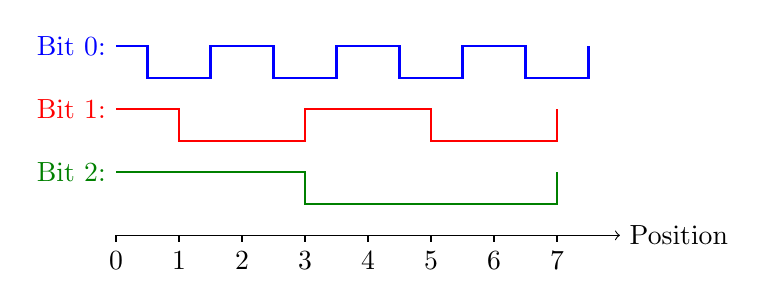
\begin{tikzpicture}[scale=0.8]
\draw[->] (0,0) -- (8,0) node[right] {Position};

% Bit 0: period 2
\draw[thick, blue] (0,3) node[left] {Bit 0:} -- (0.5,3) -- (0.5,2.5) -- (1.5,2.5) -- (1.5,3) -- (2.5,3) -- (2.5,2.5) -- (3.5,2.5) -- (3.5,3) -- (4.5,3) -- (4.5,2.5) -- (5.5,2.5) -- (5.5,3) -- (6.5,3) -- (6.5,2.5) -- (7.5,2.5) -- (7.5,3);

% Bit 1: period 4
\draw[thick, red] (0,2) node[left] {Bit 1:} -- (1,2) -- (1,1.5) -- (3,1.5) -- (3,2) -- (5,2) -- (5,1.5) -- (7,1.5) -- (7,2);

% Bit 2: period 8
\draw[thick, green!50!black] (0,1) node[left] {Bit 2:} -- (3,1) -- (3,0.5) -- (7,0.5) -- (7,1);

\foreach \x in {0,1,...,7} {
    \draw (\x, 0) -- (\x, -0.1) node[below] {\x};
}
\end{tikzpicture}
\end{center}

This multi-scale structure is exactly what we want! Each bit provides a different level of positional information:
\begin{itemize}
\item \textbf{High-frequency bits:} Distinguish nearby positions
\item \textbf{Low-frequency bits:} Distinguish distant positions
\end{itemize}

\subsection{Adapting Binary to Embeddings}

We can create a $d$-dimensional positional encoding where each dimension is a ``bit'' with a different frequency. For dimension $j$, we use period $2^{j+1}$:

\[
\mathbf{P}_{i,j} = \text{bit}_j(i) = \begin{cases}
1 & \text{if } \lfloor i / 2^j \rfloor \text{ is odd} \\
0 & \text{otherwise}
\end{cases}
\]

For a 4-dimensional encoding of positions 0-7:

\begin{center}
\begin{tabular}{c|cccc}
Position & Dim 0 & Dim 1 & Dim 2 & Dim 3 \\
\hline
0 & 0 & 0 & 0 & 0 \\
1 & 1 & 0 & 0 & 0 \\
2 & 0 & 1 & 0 & 0 \\
3 & 1 & 1 & 0 & 0 \\
4 & 0 & 0 & 1 & 0 \\
5 & 1 & 0 & 1 & 0 \\
6 & 0 & 1 & 1 & 0 \\
7 & 1 & 1 & 1 & 0 \\
\end{tabular}
\end{center}

\subsection{What Works}

\begin{itemize}
\item \textbf{Multi-scale:} Different dimensions capture different granularities of position
\item \textbf{Unique:} Each position has a unique binary pattern (for $d \geq \log_2 n$)
\item \textbf{Local and global distinction:} High-frequency dimensions distinguish neighbors; low-frequency dimensions distinguish distant positions
\item \textbf{Bounded:} Values are in $\{0, 1\}$
\end{itemize}

\subsection{What Fails}

\begin{tcolorbox}[colback=red!5!white, colframe=red!75!black, title=Critical Problem: Discontinuity]
Binary values jump abruptly from 0 to 1. Consider the transition from position 3 to position 4:

\textbf{Position 3:} [1, 1, 0, 0]

\textbf{Position 4:} [0, 0, 1, 0]

\textbf{Hamming distance:} 3 bits changed!

Despite being adjacent positions, their encodings are very different (3 dimensions flipped). This violates our smoothness requirement.

\textbf{Why this matters:} Neural networks trained with gradient descent rely on smooth, continuous functions. Sharp discontinuities make optimization difficult. If position 3 and position 4 have radically different encodings, the network cannot smoothly interpolate between them.
\end{tcolorbox}

\textbf{Additional issue:}
\begin{itemize}
\item \textbf{No useful linear transformation structure:} While binary representations are mathematically elegant for counting, they do not transform linearly in ways that dot products can exploit. Consider: to shift from position 3 [1,1,0,0] to position 4 [0,0,1,0], you flip 3 bits. But to shift from position 4 [0,0,1,0] to position 5 [1,0,1,0], you flip only 1 bit. There is no single rotation matrix $\mathbf{R}$ such that $\mathbf{p}_{i+1} = \mathbf{R} \mathbf{p}_i$ for all $i$. This violates our constraint that position shifts should be position-independent linear transformations.
\end{itemize}

\textbf{Lesson learned:} We need the multi-scale frequency structure of binary encoding, but with \emph{smooth, continuous} functions.

\section{Attempt 3: Smoothed Multi-Scale Encoding}

\subsection{The Key Insight: Replace Bits with Waves}

Instead of square waves (0/1 bits) that jump abruptly, what if we use \textbf{smooth oscillating functions} that vary continuously?

The natural choice: \textbf{sine and cosine waves!}

\begin{center}
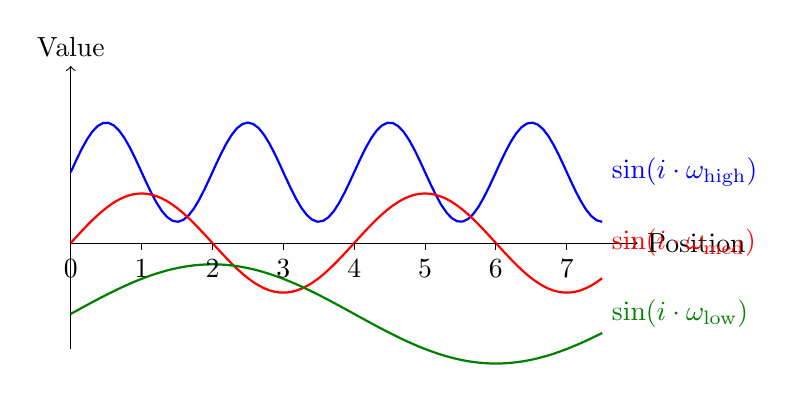
\begin{tikzpicture}[scale=0.9]
\draw[->] (0,0) -- (8,0) node[right] {Position};
\draw[->] (0,-1.5) -- (0,2.5) node[above] {Value};

% High frequency (like bit 0)
\draw[thick, blue, domain=0:7.5, samples=100] plot (\x, {1 + 0.7*sin(2*pi*\x/2 r)});
\node[blue, right] at (7.5, 1) {$\sin(i \cdot \omega_{\text{high}})$};

% Medium frequency (like bit 1)
\draw[thick, red, domain=0:7.5, samples=100] plot (\x, {0 + 0.7*sin(2*pi*\x/4 r)});
\node[red, right] at (7.5, 0) {$\sin(i \cdot \omega_{\text{med}})$};

% Low frequency (like bit 2)
\draw[thick, green!50!black, domain=0:7.5, samples=100] plot (\x, {-1 + 0.7*sin(2*pi*\x/8 r)});
\node[green!50!black, right] at (7.5, -1) {$\sin(i \cdot \omega_{\text{low}})$};

\foreach \x in {0,1,...,7} {
    \draw (\x, 0) -- (\x, -0.1) node[below] {\x};
}
\end{tikzpicture}
\end{center}

Each ``bit'' becomes a sinusoid with a different frequency:
\begin{itemize}
\item \textbf{High frequency $\omega_{\text{high}}$:} Oscillates rapidly, like Bit 0
\item \textbf{Medium frequency $\omega_{\text{med}}$:} Oscillates moderately, like Bit 1
\item \textbf{Low frequency $\omega_{\text{low}}$:} Oscillates slowly, like Bit 2
\end{itemize}

Now adjacent positions have \emph{smoothly varying} encodings!

\subsection{What Works}

\begin{itemize}
\item \textbf{Smooth and continuous:} No abrupt jumps between adjacent positions
\item \textbf{Multi-scale:} Different frequencies capture different positional granularities
\item \textbf{Bounded:} Sine values stay in $[-1, 1]$
\item \textbf{Generalizes:} Can evaluate at any position, even those not seen during training
\end{itemize}

\subsection{Remaining Questions}

This is promising, but we still need to answer:
\begin{enumerate}
\item How do we choose the frequencies $\omega_j$?
\item Why use \emph{both} sine and cosine for each frequency?
\item How does this relate to our constraint about rotations?
\end{enumerate}

\section{The Rotation Connection: Why Sine and Cosine Pairs?}

\subsection{Rotations, Angles, and Trigonometry}

Recall our constraint: positional encoding should be compatible with rotations. In 2D, a rotation by angle $\theta$ is:
\[
\begin{bmatrix}
\cos\theta & -\sin\theta \\
\sin\theta & \cos\theta
\end{bmatrix}
\]

Rotations are parameterized by \textbf{angles}, and angles are naturally expressed using \textbf{sine and cosine}.

\begin{tcolorbox}[colback=blue!5!white, colframe=blue!50!black, title=The Trigonometric Identity]
For any angle $\alpha$, the pair $(\cos\alpha, \sin\alpha)$ represents a point on the unit circle. This pair completely specifies the angle $\alpha$ (up to $2\pi$ periodicity).

Conversely, given a pair $(\cos\alpha, \sin\alpha)$, we can recover $\alpha$ using $\arctan(\sin\alpha / \cos\alpha)$.

The sine and cosine pair provides a \emph{redundant but robust} encoding of the angle.
\end{tcolorbox}

\subsection{Why Pairs of Sine and Cosine?}

If we use only sine (or only cosine), we lose information. Consider $\sin(\alpha)$:
\begin{itemize}
\item $\sin(30°) = \sin(150°) = 0.5$ $\rightarrow$ ambiguity!
\item We cannot uniquely determine the angle from sine alone
\end{itemize}

But the \emph{pair} $(\sin\alpha, \cos\alpha)$ uniquely determines $\alpha$ in $[0, 2\pi)$:
\begin{itemize}
\item $(\sin 30°, \cos 30°) = (0.5, 0.866)$
\item $(\sin 150°, \cos 150°) = (0.5, -0.866)$
\item These are distinct!
\end{itemize}

\textbf{Phase coverage:} Sine and cosine are 90 degrees out of phase. Together, they provide complete information about position along a periodic cycle.

\begin{center}
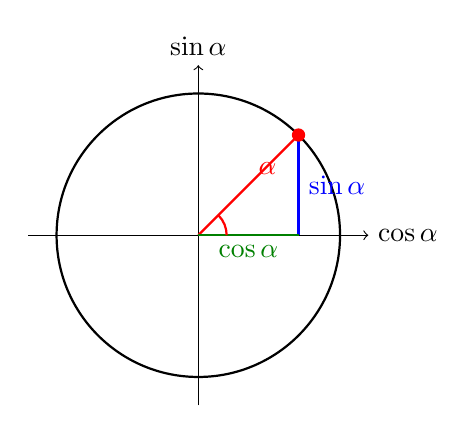
\begin{tikzpicture}[scale=1.2]
% Unit circle
\draw[thick] (0,0) circle (1.5);
\draw[->] (-1.8,0) -- (1.8,0) node[right] {$\cos\alpha$};
\draw[->] (0,-1.8) -- (0,1.8) node[above] {$\sin\alpha$};

% Angle alpha
\draw[thick, red] (0,0) -- (45:1.5) node[midway, above right] {$\alpha$};
\draw[thick, blue] (45:1.5) -- (45:1.5 |- 0,0) node[midway, right] {$\sin\alpha$};
\draw[thick, green!50!black] (0,0) -- (45:1.5 |- 0,0) node[midway, below] {$\cos\alpha$};

% Arc for angle
\draw[thick, red] (0.3,0) arc (0:45:0.3);

% Point on circle
\fill[red] (45:1.5) circle (2pt);
\end{tikzpicture}
\end{center}

\subsection{Each Frequency Gets a Sine-Cosine Pair}

For each frequency $\omega_j$, we use \emph{both} sine and cosine to encode position $i$:
\begin{align}
\text{Dimension } 2j &: \sin(i \cdot \omega_j) \\
\text{Dimension } 2j+1 &: \cos(i \cdot \omega_j)
\end{align}

This means:
\begin{itemize}
\item Dimensions come in pairs: (Dim 0, Dim 1), (Dim 2, Dim 3), (Dim 4, Dim 5), ...
\item Each pair encodes position using a different frequency $\omega_j$
\item Within each pair, sine and cosine provide complementary information
\end{itemize}

\textbf{Total dimensions:} For $d$ dimensions, we have $d/2$ frequencies.

\section{The Final Design: Sinusoidal Positional Encoding}

\subsection{Choosing Frequencies: Geometric Progression}

We want frequencies that span from high (distinguishing neighbors) to low (distinguishing distant positions). The Transformer uses a \textbf{geometric progression}:
\[
\omega_j = \frac{1}{10000^{2j/d}}
\]

As $j$ increases from $0$ to $d/2 - 1$:
\begin{itemize}
\item $\omega_0 = \frac{1}{10000^{0}} = 1$ (highest frequency, shortest wavelength)
\item $\omega_{d/2-1} = \frac{1}{10000^{(d-2)/d}} \approx \frac{1}{10000}$ (lowest frequency, longest wavelength)
\end{itemize}

The wavelength (period) of each frequency grows geometrically:
\begin{align}
\lambda_j = \frac{2\pi}{\omega_j} = 2\pi \cdot 10000^{2j/d}
\end{align}

\begin{tcolorbox}[colback=yellow!5!white, colframe=orange!50!black, title=The Magic Number: Why 10000?]
The choice of 10000 as the base is a hyperparameter designed to ensure good coverage of the expected sequence lengths.

For the lowest frequency dimension ($j = d/2 - 1$):
\[
\lambda_{\max} = 2\pi \cdot 10000 \approx 62832
\]

This extremely long wavelength means:
\begin{itemize}
\item For sequences up to several thousand tokens, the lowest frequency dimensions provide \textit{nearly linear} global positional information (the sine/cosine barely complete one cycle)
\item For sequences around 512-2048 tokens (common in the original Transformer), position 0 and position 2048 receive clearly distinct global positional encodings
\item If 10000 were much smaller (e.g., 100), the longest wavelength would be only $\sim$628 tokens, and positions beyond that would start repeating patterns
\end{itemize}

\textbf{Design principle:} Choose the base such that $\lambda_{\max}$ is significantly longer than your maximum expected sequence length, ensuring unique global positional information across the entire sequence.
\end{tcolorbox}

\textbf{Intuition:} This mirrors how we use different ``magnitudes'' in number systems:
\begin{itemize}
\item High frequencies ($j$ small): Like ones, tens $\rightarrow$ distinguish nearby positions
\item Low frequencies ($j$ large): Like hundreds, thousands $\rightarrow$ distinguish distant positions
\end{itemize}

\subsection{The Complete Formula}

For position $i$ and dimension $j$:
\begin{align}
\mathbf{P}_{i,2j} &= \sin\left(\frac{i}{10000^{2j/d}}\right) \\
\mathbf{P}_{i,2j+1} &= \cos\left(\frac{i}{10000^{2j/d}}\right)
\end{align}

\textbf{Concrete example:} For $d = 512$ dimensions and position $i = 50$:

\begin{center}
\begin{tabular}{c|c|c|c}
$j$ & Frequency $\omega_j$ & $\mathbf{P}_{50,2j} = \sin(50 \omega_j)$ & $\mathbf{P}_{50,2j+1} = \cos(50 \omega_j)$ \\
\hline
0 & 1.0000 & $\sin(50) = -0.262$ & $\cos(50) = 0.965$ \\
10 & 0.6310 & $\sin(31.55) = -0.031$ & $\cos(31.55) = 0.999$ \\
50 & 0.1585 & $\sin(7.92) = 0.997$ & $\cos(7.92) = -0.077$ \\
100 & 0.0398 & $\sin(1.99) = 0.910$ & $\cos(1.99) = -0.415$ \\
255 & 0.0001 & $\sin(0.005) = 0.005$ & $\cos(0.005) = 1.000$ \\
\end{tabular}
\end{center}

Notice how low-$j$ dimensions change rapidly with position (large arguments to sine/cosine), while high-$j$ dimensions change slowly.

\subsection{How Positional Encoding is Used}

The positional encoding is \textbf{added} to token embeddings:
\[
\mathbf{X}_{\text{input}} = \mathbf{E} + \mathbf{P}
\]

where:
\begin{itemize}
\item $\mathbf{E} \in \mathbb{R}^{n \times d}$ is the token embedding matrix
\item $\mathbf{P} \in \mathbb{R}^{n \times d}$ is the positional encoding matrix
\item $\mathbf{X}_{\text{input}} \in \mathbb{R}^{n \times d}$ goes into the first Transformer layer
\end{itemize}

\textbf{Why add, not concatenate?}
\begin{itemize}
\item \textbf{Fixed dimensionality:} Keeps model dimension at $d$, avoiding dimension increase and extra parameters
\item \textbf{Learnable mixing:} Subsequent layers can learn how to weight semantic vs. positional information
\item \textbf{Efficiency:} No dimension increase means fewer parameters in all attention layers
\end{itemize}

\begin{tcolorbox}[colback=blue!5!white, colframe=blue!50!black, title=How Does Addition Work? Disentanglement in High Dimensions]
A natural question: if we simply add $\mathbf{e}_i + \mathbf{p}_i$, how does the model distinguish between semantic and positional information?

\textbf{The high-dimensional magic:} In a 512-dimensional space, there is enormous capacity for different types of information to occupy different subspaces or ``directions.'' The network learns to allocate dimensions appropriately:
\begin{itemize}
\item Some dimensions primarily encode semantic information (word meaning)
\item Some dimensions primarily encode positional information
\item The attention mechanism and subsequent layers learn to extract what they need
\end{itemize}

\textbf{Geometric intuition:} Addition acts as a \textit{perturbation} or \textit{nudge} to the semantic vector. Rather than replacing semantic information, positional encoding shifts each embedding in the space while preserving the overall semantic relationships. The model learns which ``nudges'' correspond to which positions.

\textbf{The learned projections matter:} The query and key projection matrices $W_Q$ and $W_K$ are learned to extract the relevant combinations of semantic and positional information for each attention head. Different heads can focus on different aspects.
\end{tcolorbox}

\textbf{Scaling in Practice:}

In the original Transformer implementation, token embeddings are scaled \textit{up} before adding positional encoding:
\[
\mathbf{X}_{\text{input}} = \mathbf{E} \cdot \sqrt{d} + \mathbf{P}
\]

\textbf{Why scale the embeddings?}
\begin{itemize}
\item Token embeddings from the embedding layer typically have values with variance $\approx 1/d$ (due to initialization)
\item After scaling by $\sqrt{d}$, embeddings have variance $\approx 1$
\item Positional encodings have bounded values in $[-1, 1]$, also with variance $\approx 1$
\item This ensures both components have similar magnitudes and contribute roughly equally
\end{itemize}

Without scaling, the positional encoding (with values in $[-1,1]$) would dominate the small embedding values, and the semantic information would be lost.

\section{The Magic: Relative Position as Rotation}

One of the most elegant properties of sinusoidal encoding is that \emph{relative positions can be expressed as linear transformations}. This means the model can easily learn to attend based on relative distances (e.g., ``look 3 tokens back'') rather than absolute positions.

\subsection{Mathematical Property}

For any fixed offset $\delta$, the positional encoding at position $i + \delta$ can be obtained from the encoding at position $i$ via a linear transformation. Specifically, for a single frequency $\omega_j = 1/10000^{2j/d}$:

\begin{equation}
\begin{bmatrix}
\mathbf{P}_{i+\delta,2j} \\
\mathbf{P}_{i+\delta,2j+1}
\end{bmatrix}
=
\begin{bmatrix}
\cos(\delta \omega_j) & \sin(\delta \omega_j) \\
-\sin(\delta \omega_j) & \cos(\delta \omega_j)
\end{bmatrix}
\begin{bmatrix}
\mathbf{P}_{i,2j} \\
\mathbf{P}_{i,2j+1}
\end{bmatrix}
\end{equation}

The $2 \times 2$ transformation matrix is a rotation matrix by angle $\delta \omega_j$. Crucially, this matrix depends only on the offset $\delta$ and the frequency $\omega_j$, \emph{not on the starting position $i$}.

\subsection{Derivation of the Rotation Property}

Let us verify this property using trigonometric identities. Starting with the positional encoding at position $i$:

\begin{align}
\mathbf{P}_{i,2j} &= \sin(i \omega_j) \\
\mathbf{P}_{i,2j+1} &= \cos(i \omega_j)
\end{align}

For position $i + \delta$:

\begin{align}
\mathbf{P}_{i+\delta,2j} &= \sin((i + \delta) \omega_j) \\
&= \sin(i \omega_j) \cos(\delta \omega_j) + \cos(i \omega_j) \sin(\delta \omega_j) \\
&= \cos(\delta \omega_j) \cdot \mathbf{P}_{i,2j} + \sin(\delta \omega_j) \cdot \mathbf{P}_{i,2j+1}
\end{align}

Similarly:

\begin{align}
\mathbf{P}_{i+\delta,2j+1} &= \cos((i + \delta) \omega_j) \\
&= \cos(i \omega_j) \cos(\delta \omega_j) - \sin(i \omega_j) \sin(\delta \omega_j) \\
&= -\sin(\delta \omega_j) \cdot \mathbf{P}_{i,2j} + \cos(\delta \omega_j) \cdot \mathbf{P}_{i,2j+1}
\end{align}

This confirms that the transformation is indeed a rotation matrix that depends only on $\delta$.

\subsection{The Clock Analogy}

Think of each frequency pair (sine, cosine) as a clock face:
\begin{itemize}
\item The position $i$ determines where the hand points on the clock.
\item Moving forward by $\delta$ positions corresponds to rotating the hand by a fixed angle $\delta \omega_j$.
\item This rotation is the same regardless of where you start on the clock: moving from 1 o'clock to 2 o'clock requires the same rotation as moving from 7 o'clock to 8 o'clock.
\end{itemize}

\begin{center}
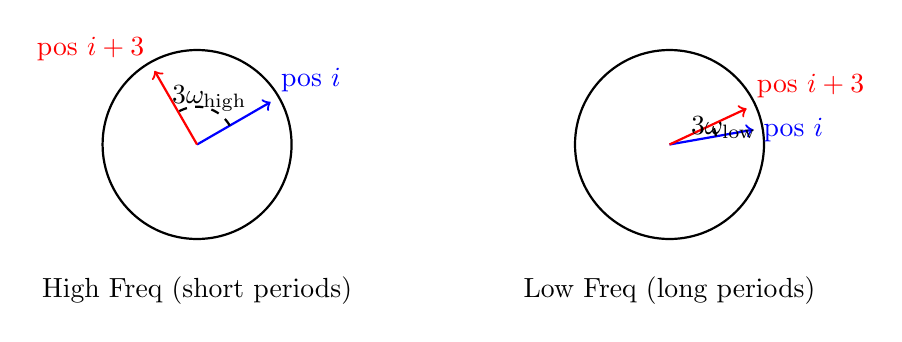
\begin{tikzpicture}[scale=1.2]
% High frequency clock (fast)
\begin{scope}[xshift=0cm]
\draw[thick] (0,0) circle (1);
\draw[thick, blue, ->] (0,0) -- (30:0.9) node[above right] {pos $i$};
\draw[thick, red, ->] (0,0) -- (120:0.9) node[above left] {pos $i+3$};
\draw[thick, dashed] (30:0.4) arc (30:120:0.4);
\node at (75:0.5) {$3\omega_{\text{high}}$};
\node[below] at (0,-1.3) {High Freq (short periods)};
\end{scope}

% Low frequency clock (slow)
\begin{scope}[xshift=5cm]
\draw[thick] (0,0) circle (1);
\draw[thick, blue, ->] (0,0) -- (10:0.9) node[right] {pos $i$};
\draw[thick, red, ->] (0,0) -- (25:0.9) node[above right] {pos $i+3$};
\draw[thick, dashed] (10:0.5) arc (10:25:0.5);
\node at (17.5:0.6) {$3\omega_{\text{low}}$};
\node[below] at (0,-1.3) {Low Freq (long periods)};
\end{scope}
\end{tikzpicture}
\end{center}

Moving forward by $\delta = 3$ positions:
\begin{itemize}
\item \textbf{High-frequency clock:} Hand rotates by a large angle $\delta \omega_{\text{high}}$ (big change)
\item \textbf{Low-frequency clock:} Hand rotates by a small angle $\delta \omega_{\text{low}}$ (small change)
\end{itemize}

The crucial insight: the rotation angle depends on $\delta$ (the offset), not on where you start ($i$).

\textbf{Moving from position 5 to 8 ($\delta=3$) gives the same rotation as moving from position 100 to 103 ($\delta=3$).}

\section{How Positional Encoding Actually Works in Attention}

We have designed an elegant positional encoding, but how does it \textit{actually} interact with the attention mechanism? Let us decompose what happens when we compute attention scores.

\subsection{Decomposing the Attention Score}

When computing attention between position $i$ (query) and position $j$ (key), we first project the combined semantic and positional vectors:
\[
\mathbf{q}_i = W_Q(\mathbf{e}_i + \mathbf{p}_i), \quad \mathbf{k}_j = W_K(\mathbf{e}_j + \mathbf{p}_j)
\]

The attention score is their dot product:
\[
\text{score}(i, j) = \mathbf{q}_i^T \mathbf{k}_j
\]

\textbf{Simplified analysis:} To understand the core mechanism, let us first ignore the learned projections ($W_Q = W_K = I$) and examine the raw dot product:
\[
\text{score}(i, j) = (\mathbf{e}_i + \mathbf{p}_i)^T (\mathbf{e}_j + \mathbf{p}_j)
\]

Expanding this product gives four terms:
\begin{align}
\text{score}(i, j) = &\underbrace{\mathbf{e}_i^T \mathbf{e}_j}_{\text{Term 1: Content-Content}} + \underbrace{\mathbf{e}_i^T \mathbf{p}_j}_{\text{Term 2: Content-Position}} \\
&+ \underbrace{\mathbf{p}_i^T \mathbf{e}_j}_{\text{Term 3: Position-Content}} + \underbrace{\mathbf{p}_i^T \mathbf{p}_j}_{\text{Term 4: Position-Position}}
\end{align}

Let us interpret each term:

\begin{enumerate}
\item \textbf{Term 1 (Content-to-Content):} $\mathbf{e}_i^T \mathbf{e}_j$

Pure semantic similarity. Does the meaning of word $i$ relate to the meaning of word $j$? This is what attention would compute without any positional information.

\item \textbf{Term 2 (Content-to-Position):} $\mathbf{e}_i^T \mathbf{p}_j$

How much does the \textit{semantic content} at position $i$ attend to a particular \textit{position} $j$? This allows content-dependent positional biases. For example: a verb might learn to attend more to positions that typically contain subjects (earlier positions).

\item \textbf{Term 3 (Position-to-Content):} $\mathbf{p}_i^T \mathbf{e}_j$

How much does the \textit{position} $i$ attend to particular \textit{semantic content} at $j$? This is the symmetric counterpart to Term 2. For example: the first position might learn to attend more to words that are typically sentence subjects.

\item \textbf{Term 4 (Position-to-Position):} $\mathbf{p}_i^T \mathbf{p}_j$

Pure positional relationship, independent of content. This term captures patterns like ``position $i$ should attend to position $i-1$'' (previous word) or ``position $i$ should attend to position $i+k$'' (word at offset $k$).
\end{enumerate}

\begin{tcolorbox}[colback=green!5!white, colframe=green!50!black, title=The Key Insight: Position-Position Term and Relative Distance]
Because of the rotation property of sinusoidal encoding, \textbf{Term 4 depends primarily on the relative distance $|i-j|$, not the absolute positions.}

Recall that for any offset $\delta$, we have:
\[
\mathbf{p}_{i+\delta} = \mathbf{R}_\delta \mathbf{p}_i
\]
where $\mathbf{R}_\delta$ is a block-diagonal rotation matrix depending only on $\delta$.

Therefore:
\[
\mathbf{p}_i^T \mathbf{p}_{i+\delta} = \mathbf{p}_i^T \mathbf{R}_\delta \mathbf{p}_i
\]

This is a function of the offset $\delta = j - i$, not the absolute position $i$. The model can learn to use this term to implement relative positional attention patterns like ``attend to the previous word'' or ``attend to words within a window.''
\end{tcolorbox}

\subsection{The Role of Learned Projection Matrices}

In practice, the attention score involves learned projections:
\[
\text{score}(i, j) = (W_Q(\mathbf{e}_i + \mathbf{p}_i))^T (W_K(\mathbf{e}_j + \mathbf{p}_j))
\]

Expanding:
\[
= (W_Q \mathbf{e}_i + W_Q \mathbf{p}_i)^T (W_K \mathbf{e}_j + W_K \mathbf{p}_j)
\]

This introduces four projected terms:
\begin{align}
\text{score}(i, j) = &(W_Q \mathbf{e}_i)^T (W_K \mathbf{e}_j) + (W_Q \mathbf{e}_i)^T (W_K \mathbf{p}_j) \\
&+ (W_Q \mathbf{p}_i)^T (W_K \mathbf{e}_j) + (W_Q \mathbf{p}_i)^T (W_K \mathbf{p}_j)
\end{align}

\textbf{The challenge:} Arbitrary learned matrices $W_Q$ and $W_K$ can obscure or break the elegant rotational structure of the positional encoding!

\begin{itemize}
\item The clean separation between semantic and positional components is no longer guaranteed
\item The position-position term $(W_Q \mathbf{p}_i)^T (W_K \mathbf{p}_j)$ no longer has a simple dependence on relative distance $i-j$
\item The network must \textit{learn} to utilize the sinusoidal structure, which is not enforced by the architecture
\end{itemize}

\textbf{What the model learns:} In practice, different attention heads learn to extract different combinations:
\begin{itemize}
\item Some heads focus primarily on semantic similarity (weighting Term 1)
\item Some heads learn positional patterns (weighting Term 4)
\item Many heads use a mixture of content and position
\end{itemize}

The flexibility is powerful, but the lack of explicit structural enforcement motivated the development of newer techniques.

\subsection{Bridge to Modern Techniques: Rotary Positional Embeddings (RoPE)}

The analysis above reveals a fundamental limitation: the learned projection matrices can break the geometric elegance of sinusoidal encoding.

\textbf{RoPE's key innovation:} Instead of adding positional information to the embeddings \textit{before} projection, RoPE applies rotations \textit{after} projection:

\begin{align}
\mathbf{q}_i &= \mathbf{R}_i (W_Q \mathbf{e}_i) \\
\mathbf{k}_j &= \mathbf{R}_j (W_K \mathbf{e}_j)
\end{align}

where $\mathbf{R}_i$ is a position-dependent rotation matrix.

When computing the attention score:
\begin{align}
\text{score}(i, j) &= \mathbf{q}_i^T \mathbf{k}_j \\
&= (W_Q \mathbf{e}_i)^T \mathbf{R}_i^T \mathbf{R}_j (W_K \mathbf{e}_j) \\
&= (W_Q \mathbf{e}_i)^T \mathbf{R}_{j-i} (W_K \mathbf{e}_j)
\end{align}

The crucial property: $\mathbf{R}_i^T \mathbf{R}_j = \mathbf{R}_{j-i}$ (rotation matrices compose by adding angles).

\textbf{The result:} The attention score depends explicitly on:
\begin{itemize}
\item The semantic content (through $W_Q \mathbf{e}_i$ and $W_K \mathbf{e}_j$)
\item The \textit{relative position} $j - i$ (through $\mathbf{R}_{j-i}$)
\end{itemize}

The rotational structure is \textbf{enforced by the architecture}, not merely provided as a signal the network might learn to use.

\textbf{Advantages of RoPE:}
\begin{itemize}
\item Better extrapolation to longer sequences (the relative position structure is explicit)
\item More parameter-efficient (no positional embedding parameters to learn)
\item Stronger inductive bias for relative position patterns
\end{itemize}

\textbf{Why sinusoidal encoding is still important:} Understanding sinusoidal PE provides the geometric intuition behind RoPE. RoPE realizes the same rotation-based relative position concept, but applies it more directly. Modern models like LLaMA, PaLM, and Mistral all use RoPE or variants.

\begin{tcolorbox}[colback=blue!5!white, colframe=blue!50!black, title=Evolution of Positional Encoding]
\textbf{Sinusoidal PE (Vaswani et al., 2017):} Add rotation-structured position encoding before projection. The model must learn to use it.

\textbf{Learned PE (BERT/GPT):} Replace fixed sinusoids with learned embeddings. More flexible but no inherent relative position structure.

\textbf{RoPE (Su et al., 2021):} Apply rotations after projection. Enforces relative position structure directly in attention computation.

\textbf{ALiBi (Press et al., 2021):} Add bias to attention scores based on distance. Simpler but less expressive.

Each approach makes different trade-offs between:
\begin{itemize}
\item \textbf{Inductive bias:} How much structure is built into the architecture?
\item \textbf{Flexibility:} Can the model learn arbitrary positional patterns?
\item \textbf{Extrapolation:} How well does it generalize to longer sequences?
\end{itemize}
\end{tcolorbox}

\section{Visualizing the Encoding}

\subsection{Heatmap Visualization}

Consider a positional encoding matrix for 60 positions and 32 dimensions:

\begin{center}
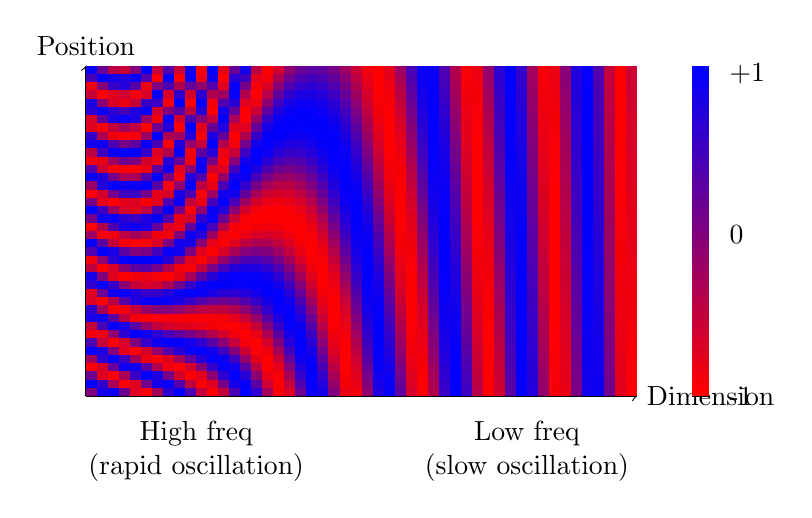
\begin{tikzpicture}[scale=0.7]
\draw[->] (0,0) -- (10,0) node[right] {Dimension};
\draw[->] (0,0) -- (0,6) node[above] {Position};

% Simulate heatmap with rectangles
% High frequency on left (small j), low frequency on right (large j)
\foreach \x in {0,0.2,...,9.8} {
    \foreach \y in {0,0.15,...,5.85} {
        \pgfmathsetmacro{\freq}{1/(1 + (\x/10)^3 * 99)}
        \pgfmathsetmacro{\val}{sin((\y*10 * \freq + \x*5) r)}
        \pgfmathsetmacro{\col}{(\val + 1) * 50}
        \fill[blue!\col!red] (\x, \y) rectangle (\x+0.2, \y+0.15);
    }
}

\node[align=center] at (2, -1) {High freq\\(rapid oscillation)};
\node[align=center] at (8, -1) {Low freq\\(slow oscillation)};

% Colorbar
\draw (11, 0) rectangle (11.3, 5.85);
\foreach \y in {0,0.15,...,5.85} {
    \pgfmathsetmacro{\col}{\y/5.85 * 100}
    \fill[blue!\col!red] (11, \y) rectangle (11.3, \y+0.15);
}
\node[right] at (11.5, 5.85) {+1};
\node[right] at (11.5, 2.925) {0};
\node[right] at (11.5, 0) {-1};
\end{tikzpicture}
\end{center}

\textbf{Observations:}
\begin{itemize}
\item \textbf{Left columns:} Tight vertical stripes (high frequency). Adjacent positions have very different values $\rightarrow$ good for local distinctions.
\item \textbf{Right columns:} Broad vertical bands (low frequency). Values change slowly across positions $\rightarrow$ good for global structure.
\item \textbf{Each row is unique:} No two positions have the same pattern across dimensions.
\end{itemize}

\subsection{Individual Dimension Traces}

Plotting how several dimensions vary with position:

\begin{center}
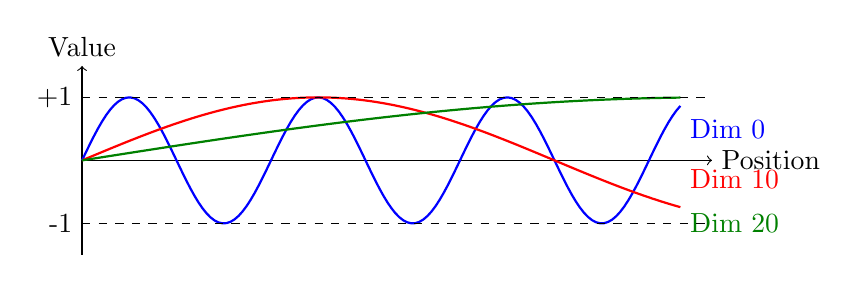
\begin{tikzpicture}[scale=0.8]
\draw[->] (0,0) -- (10,0) node[right] {Position};
\draw[->] (0,-1.5) -- (0,1.5) node[above] {Value};

% Dimension 0 (very high frequency)
\draw[thick, blue, domain=0:9.5, samples=150] plot (\x, {sin(2*pi*\x/3 r)});

% Dimension 10 (medium frequency)
\draw[thick, red, domain=0:9.5, samples=150] plot (\x, {sin(2*pi*\x/15 r)});

% Dimension 20 (low frequency)
\draw[thick, green!50!black, domain=0:9.5, samples=150] plot (\x, {sin(2*pi*\x/40 r)});

\node[blue, right] at (9.5, 0.5) {Dim 0};
\node[red, right] at (9.5, -0.3) {Dim 10};
\node[green!50!black, right] at (9.5, -1.0) {Dim 20};

\draw[dashed] (0,1) -- (10,1);
\draw[dashed] (0,-1) -- (10,-1);
\node[left] at (0,1) {+1};
\node[left] at (0,-1) {-1};
\end{tikzpicture}
\end{center}

\textbf{Interpretation:}
\begin{itemize}
\item \textbf{Dim 0 (blue):} Completes multiple cycles $\rightarrow$ changes rapidly, distinguishes every position
\item \textbf{Dim 10 (red):} Moderate oscillation $\rightarrow$ captures medium-range structure
\item \textbf{Dim 20 (green):} Slow variation $\rightarrow$ encodes coarse position (beginning vs. end)
\end{itemize}

Together, these dimensions provide a multi-resolution ``fingerprint'' of position.

\section{Satisfying All Design Goals}

Let us verify that sinusoidal encoding meets all our requirements:

\begin{enumerate}
\item \textbf{Uniqueness:} Each position has a unique $d$-dimensional vector (sine/cosine combinations are unique for reasonable sequence lengths).

\item \textbf{Determinism:} The encoding is a fixed mathematical function, always producing the same output for the same position.

\item \textbf{Bounded Range:} All values lie in $[-1, 1]$, ensuring numerical stability.

\item \textbf{Generalization:} The formula works for any position $i$, including those beyond the training sequence length. Sine and cosine are defined for all real arguments.

\item \textbf{Distance Awareness:} Multi-scale frequencies distinguish both short distances (high $\omega_j$) and long distances (low $\omega_j$).

\item \textbf{Smooth Transitions:} Sine and cosine are infinitely differentiable $\rightarrow$ gradients flow smoothly during training.

\item \textbf{Linear Transformability:} Shifting by $\delta$ positions corresponds to a simple rotation (linear transformation) that is independent of the starting position.

\item \textbf{Norm Preservation:} All positional encodings have the same norm: $\|\mathbf{p}_i\| = \|\mathbf{p}_j\|$ for all positions $i, j$.
\end{enumerate}

\begin{tcolorbox}[colback=green!5!white, colframe=green!50!black, title=The Elegant Solution]
Sinusoidal positional encoding achieves all design goals by:
\begin{itemize}
\item Using \textbf{multi-scale frequencies} (like binary encoding) for different granularities
\item Using \textbf{smooth sinusoids} (not discrete bits) for gradient-based optimization
\item Using \textbf{sine-cosine pairs} (not single functions) to enable rotation-based relative positions
\item Using \textbf{geometric frequency progression} to span from local to global scales
\end{itemize}

The design elegantly balances mathematical rigor (rotation invariance), engineering pragmatism (bounded values, differentiability), and representational power (multi-scale structure).
\end{tcolorbox}

\section{Connection to Fourier Analysis}

\subsection{Positional Encoding as Fourier Features}

The sinusoidal encoding can be understood through the lens of \textbf{Fourier features}. In Fourier analysis, complex signals are decomposed into sums of simple sinusoids at different frequencies.

Our positional encoding maps the scalar position $i$ to a high-dimensional feature vector:
\[
i \rightarrow \left[\sin(\omega_0 i), \cos(\omega_0 i), \sin(\omega_1 i), \cos(\omega_1 i), \ldots, \sin(\omega_{d/2-1} i), \cos(\omega_{d/2-1} i)\right]
\]

This is analogous to computing a Fourier transform of the position signal using a discrete set of basis frequencies $\{\omega_0, \omega_1, \ldots, \omega_{d/2-1}\}$.

\textbf{Why this works:} Functions that are difficult to represent in the original input space (position as a scalar) can become linearly separable or easier to model in the Fourier-transformed feature space. The multiple frequencies allow the network to capture both rapid variations (high frequencies) and gradual trends (low frequencies) in how position affects the output.

\subsection{The Frequency Spectrum}

The choice of frequencies $\omega_j = 10000^{-2j/d}$ creates a logarithmically-spaced frequency spectrum:

\begin{center}
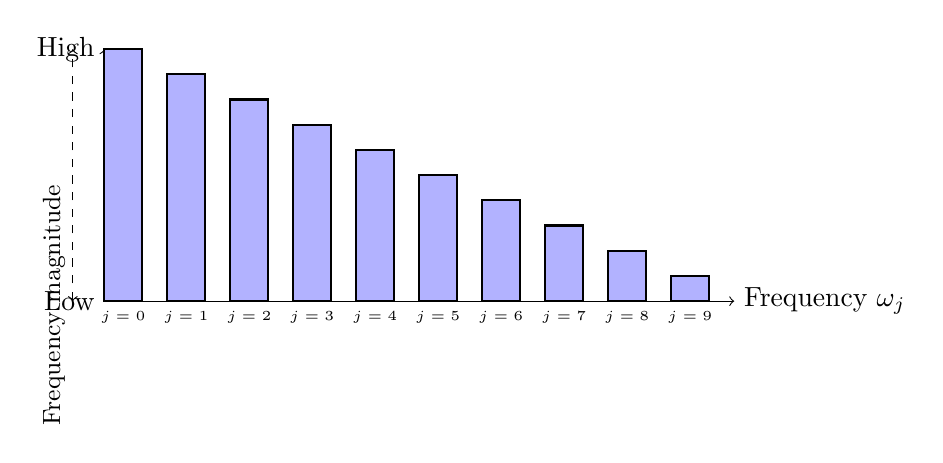
\begin{tikzpicture}[scale=0.8]
\draw[->] (0,0) -- (10,0) node[right] {Frequency $\omega_j$};
\draw[->] (0,0) -- (0,4) node[above] {};

% Frequency bars (log scale)
\foreach \j in {0,1,...,9} {
    \pgfmathsetmacro{\height}{4 - \j*0.4}
    \pgfmathsetmacro{\freq}{1/(10^(\j/5))}
    \draw[thick, fill=blue!30] (\j, 0) rectangle (\j+0.6, \height);
    \node[below, font=\tiny] at (\j+0.3, 0) {$j=\j$};
}

\node[left] at (0, 4) {High};
\node[left] at (0, 0) {Low};
\draw[<->, dashed] (-0.5, 0) -- (-0.5, 4);
\node[left, rotate=90, font=\small] at (-0.8, 2) {Frequency magnitude};
\end{tikzpicture}
\end{center}

This logarithmic spacing ensures:
\begin{itemize}
\item Coverage of many octaves (frequency doublings)
\item Efficient use of dimensions (not wasting dimensions on redundant frequencies)
\item Natural analogy to how humans perceive scale (logarithmic perception)
\end{itemize}

\section{Summary}

We have built up sinusoidal positional encoding through a progression of ideas:

\begin{enumerate}
\item \textbf{Started with geometric constraints:} Positional encoding must interact constructively with semantics, preserve norms, and enable position-independent linear transformations.

\item \textbf{Attempt 1 (Linear weights):} All positions point in the same direction, violates norm preservation, no useful geometric structure.

\item \textbf{Attempt 2 (Binary encoding):} Multi-scale structure but discontinuous jumps and no useful linear transformation for dot products.

\item \textbf{Attempt 3 (Smooth oscillations):} Replace discrete bits with continuous sinusoids for gradient-based learning.

\item \textbf{Rotation insight:} Sine-cosine pairs naturally parameterize rotations, and relative position shifts become rotation matrices.

\item \textbf{Final design:} Sinusoidal functions with geometrically-spaced frequencies (base 10000), using sine-cosine pairs for each frequency.

\item \textbf{How it works in practice:} Decomposing attention scores reveals four interaction terms (content-content, content-position, position-content, position-position). The rotation property ensures position-position term depends on relative distance.

\item \textbf{Modern evolution:} RoPE enforces the rotation structure architecturally rather than expecting the network to learn it.
\end{enumerate}

\textbf{Key mathematical properties:}
\begin{itemize}
\item Bounded values: $\mathbf{P}_{i,j} \in [-1, 1]$
\item Multi-scale representation: frequencies from $\omega_0 = 1$ to $\omega_{d/2-1} \approx 10^{-4}$
\item Rotation structure: Relative position $\delta$ corresponds to rotation by angle $\delta \omega_j$
\item Translation invariance: The transformation from position $i$ to $i+\delta$ is the same as from $j$ to $j+\delta$
\item Norm preservation: $\|\mathbf{p}_i\| = \|\mathbf{p}_j\|$ for all positions
\end{itemize}

\begin{tcolorbox}[colback=yellow!5!white, colframe=orange!50!black, title=Generalization and Limitations]
\textbf{Strengths:}
\begin{itemize}
\item The sinusoidal formula can be evaluated for any sequence length, even those never seen during training
\item The multi-scale structure provides both local and global positional information
\item No learned parameters needed for the encoding itself
\end{itemize}

\textbf{Limitations (Extrapolation):}
\begin{itemize}
\item While sinusoids are \textit{defined} for all lengths, model performance often degrades on sequences much longer than training lengths
\item If trained only on sequences up to length 512, the model may not have learned to effectively utilize the very low-frequency dimensions that would distinguish positions 512-2048
\item The learned projection matrices ($W_Q, W_K$) may not generalize well to positional patterns outside the training distribution
\item This motivated research into better extrapolation methods (RoPE, ALiBi, position interpolation)
\end{itemize}

\textbf{Practical recommendation:} If you need to handle sequences significantly longer than training sequences, consider:
\begin{itemize}
\item Using RoPE or ALiBi instead of sinusoidal PE
\item Position interpolation (scaling positions to fit training range)
\item Training on longer sequences, even if rarely
\end{itemize}
\end{tcolorbox}

This elegant design satisfies our geometric constraints while providing a mathematically principled and interpretable way to inject positional information into self-attention, making Transformers possible. The progression from sinusoidal PE to RoPE shows how understanding the geometric principles leads to architectural improvements.
\end{document}
